% Created 2016-08-17 Wed 14:38
\documentclass[tikz]{standalone}

\usepackage[utf8]{inputenc}
\usepackage[T1]{fontenc}

\usepackage{circledsteps}

\RequirePackage{xcolor}

%% HPI color definitions according to the design manual
% These do not exactly match the RGB values used in the Powerpoint slide master due to unknown reasons
\definecolor{hpiyellow}{RGB}{246,168,0}
\definecolor{hpiorange}{RGB}{221,97,8}
\definecolor{hpired}{RGB}{177,6,58}
\definecolor{hpigray}{RGB}{90,96,101}
\definecolor{hpiblue}{RGB}{0,122,158}


\renewcommand{\sfdefault}{neosans}
% Different font weights for neosans
\newcommand{\textl}[1]{{\fontseries{l}\selectfont #1}} % light
\newcommand{\textm}[1]{{\fontseries{m}\selectfont #1}} % medium, same as default weight
\newcommand{\textsb}[1]{{\fontseries{sb}\selectfont #1}} % semibold
\newcommand{\textmb}[1]{{\fontseries{mb}\selectfont #1}} % bold, same as \textbf
\newcommand{\texteb}[1]{{\fontseries{eb}\selectfont #1}} % extra bold
\newcommand{\textub}[1]{{\fontseries{ub}\selectfont #1}} % ultra bold

\tikzset{every picture/.style={/utils/exec={\sffamily}}}
\tikzset{flipflop RSflanke/.style={
  flipflop,
  flipflop def={t1=S, t2=C, c2=1, t3=R, t6=Q, t4={\ctikztextnot{Q}}}
}}


\tikzset{
  mechanicalSwitch/.pic={
    \coordinate (-inUp) at (135:2); 
    \coordinate (-inDown) at (235:2);
    \coordinate (-out) at (2,0);
    \coordinate (-center) at (0,0);
    
    \draw (0,0) circle [radius = 2cm];
    \draw [fill=gray!20] (0,0) circle [radius = 0.2cm];

    \draw (0, 0) -- (2, 0);
    \draw (135:.8) -- (135:2); 
    \draw (225:.8) -- (225:2); 

    \draw [fill=gray!20] (2, 0) circle [radius=0.05cm]; 
    \draw [fill=gray!20] (135:2) circle [radius=0.05cm]; 
    \draw [fill=gray!20] (225:2) circle [radius=0.05cm]; 

    
    \draw [thick] (0,0) -- (175:1.5); 

    \draw [dashed, <->, domain=135:225] plot ({cos(\x)}, {sin(\x)}); 
  },
  mechanicalSwitchClosed/.pic={
    \coordinate (-inUp) at (135:2); 
    \coordinate (-inDown) at (255:2);
    \coordinate (-out) at (2,0);
    \coordinate (-center) at (0,0);
    \draw (0,0) circle [radius = 2cm];
    \draw [fill=gray!20] (0,0) circle [radius = 0.2cm];

    \draw (0, 0) -- (2, 0);
    \draw (135:.8) -- (135:2); 
    \draw (225:.8) -- (225:2); 

    \draw [fill=gray!20] (2, 0) circle [radius=0.05cm]; 
    \draw [fill=gray!20] (135:2) circle [radius=0.05cm]; 
    \draw [fill=gray!20] (225:2) circle [radius=0.05cm]; 

    
    \draw [thick] (0,0) -- (135:2); 

    \draw [dashed, <->, domain=135:225] plot ({cos(\x)}, {sin(\x)}); 
  }
}


\usetikzlibrary{calc}
\usetikzlibrary{positioning}


\usetikzlibrary {decorations.pathreplacing}

\begin{document}

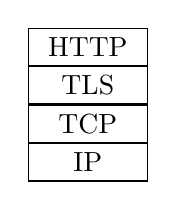
\begin{tikzpicture}[every node/.style={draw, minimum width=10ex}, node distance=0pt]
  \label{page:quic:http_tcp_stack}

  \node (http) {HTTP}; 
    \node [below=of http] (tls) {TLS}; 
    \node [below=of tls] (tcp) {TCP}; 
    \node [below=of tcp] (ip) {IP}; 
  \end{tikzpicture}

  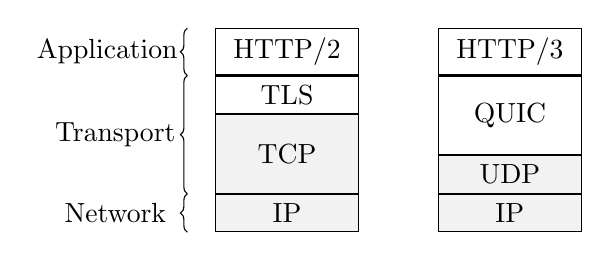
\begin{tikzpicture}[every node/.style={draw, minimum width=12ex}, node distance=0pt]
  \label{page:quic:http3_stack}
  
  \node (http2) {HTTP/2}; 
  \node [below=of http2] (tls) {TLS}; 
  \node [below=of tls, minimum height=1cm, fill=gray!10] (tcp) {TCP}; 
  \node [below=of tcp, fill=gray!10] (ip) {IP}; 

  \node [right=1cm of http2] (http3) {HTTP/3}; 
  \node [below=of http3, minimum height=1cm] (quic) {QUIC}; 
  \node [below=of quic, fill=gray!10] (udp) {UDP}; 
  \node [below=of udp, fill=gray!10] (ip2) {IP}; 

  \draw [decorate, decoration={brace,raise=10pt,mirror}] (http2.north west)  to node [midway,align=right, anchor=east, draw=none, xshift=-10pt] {Application} (http2.south west) ;

  \draw [decorate, decoration={brace,raise=10pt,mirror}] (tls.north west)  to node [midway,align=right, anchor=east, draw=none, xshift=-10pt] {Transport} (tcp.south west) ;

  \draw [decorate, decoration={brace,raise=10pt,mirror}] (ip.north west)  to node [midway,align=right, anchor=east, draw=none, xshift=-10pt] {Network} (ip.south west) ;  
  
  \end{tikzpicture}


\end{document}